\documentclass[conference]{IEEEtran}
% \IEEEoverridecommandlockouts
% The preceding line is only needed to identify funding in the first footnote. If that is unneeded, please comment it out.
\usepackage{cite}
\usepackage{amsmath,amssymb,amsfonts}
\usepackage{algorithmic}
\usepackage{graphicx}
\usepackage{siunitx}
\usepackage{textcomp}
\usepackage{xcolor}
\usepackage{multirow}
\usepackage{url}
\usepackage{epstopdf}
\usepackage{placeins}
\usepackage[inkscapeformat=png]{svg}
\usepackage[font=small,labelfont=bf]{caption}

\epstopdfDeclareGraphicsRule{.gif}{png}{.png}{convert gif:#1 png:\OutputFile}
\AppendGraphicsExtensions{.gif}

\def\BibTeX{{\rm B\kern-.05em{\sc i\kern-.025em b}\kern-.08em
    T\kern-.1667em\lower.7ex\hbox{E}\kern-.125emX}}
\begin{document}

\title{Convolutional Neural Network on CIFAR-10}

\author{\IEEEauthorblockN{Mihai Bojescu}
\IEEEauthorblockA{\textit{Master in Artificial Intelligence and Optimisation} \\
\textit{Faculty of Computer Science of University ``Alexandru Ioan Cuza'' of Iași}\\
Iași, Romania \\
bojescu.mihai@gmail.com}
}

\maketitle


\begin{abstract}
This document contains details on a Convolutional Neural Network such as its structure, how each layer contributes to the
output, how the forward function works and how the gradient flow works. The document also details the experiments performed
using the given neural network.
\end{abstract}

\begin{IEEEkeywords}
neural network, convolution, convolutional neural network, nn, cnn, gradient flow, forward function
\end{IEEEkeywords}


\section{Introduction}
This document details the structure of the Convolutional Neural Network used in this project, layer initialisation, the steps
that are performed in the $forward$ function, the gradient flow of the project, results of the project and a comparison between
the current project and the previous one. This project is built on top of the previous one, which would mean this project
is a continuation of the work and refinement of the previous project.

\section{Layers}
The Convolutional Neural Network model in this project contains 8 layers:

\begin{enumerate}
    \item 3 convolutional layers
    \item 3 max-pool 2d layers
    \item 2 dropout layers
    \item 2 fully-connected layers
\end{enumerate}

In the following subsections, each layer will be sumarised.

\subsection{Convolutional layers}
The convolutional layers play the most important role in improving the accuracy of the model. They account to an increase
in the accuracy (compared to the previous project) of ~34.5\%. Due to the way they work, they are quintesential to building
accurate models that can be used on image-datasets such as CIFAR-10 or MNIST.

The network includes 3 convolutional layers - $self.conv1$, $self.conv2$, $self.conv3$ - in the hopes that this would drive
the accuracy higher. After a convolutional layer is applied, the results go through a MaxPool2d layer. The number of layers
was chosen as a compromise between speed and accuracy.

\subsection{MaxPool2d layers}
The results of the convolutions are passed through MaxPool2d layers in order to scale-down the data. This makes the data
faster to process.

The project's model contains 3 MaxPool2d layers, one for each convolutional layer.

\subsection{Dropout layers}
Dropout layers contribute to regularization by introducing randomisation during training, preventing the model from relying
too heavily on specific activations. The stochastic nature of dropout contributes to a more robust and generalizable model.

In this project, 2 dropout layers - $self.dropout1$, $self.dropout2$ - were added for this reason.

\subsection{Fully-connected layers}
The fully-connected layers in this project's model take the flattened results of the convolutions, and multiplies them with
each the matrix of each layer. The results are passed through a ReLU activation function, and then are passed to the dropout
layers.

In this project, 3 fully-connected layers - $self.fc1$, $self.fc2$, $self.fc3$ - are used.

\section{Initialisation}
The model can be initialised in two ways:

\begin{enumerate}
    \item randomly, when in training mode
    \item using pre-existing weights and biases, when running in inference mode
\end{enumerate}

\subsection{Random initialisation}
When the model is run in training mode, the weights and biases of the layers are selected at random. Since the fully-connected
layers are passed through a ReLU activation function, they are initialised using the Kaiming Uniform initialisation function. 

\subsection{Initialisation using pre-existing weights and biases}
The model was trained multiple times. In order to be evaluated, a Python inference script - $inference.py$ - ran by a bash script
- $run\_inference.sh$ - was added. The scripts preloads weights and biases available from previous training sessions, thus,
the weights and biases are not random.

\section{The forward function}
The forward function of the model runs in multiple steps:

\begin{enumerate}
    \item ensure the data is on the specified device
    \item pass the data through the 3 max-pooled convolutional layers
    \item flatten the data in order to pass it to the fully-connected layers
    \item pass the data through the 3 ReLU-activated-fully-connected layers, while running dropout between each layer
\end{enumerate}

The steps were explained in the $Layers$ section above.

\section{Gradients flow}

\subsection{Forward pass}
The input data is fed through the convolutional layers, activation functions, and pooling layers during the forward pass.

Dropout layers, such as self.dropout1 and self.dropout2, are applied after the first and second fully connected layers, respectively.

The dropout layers randomly set a fraction of the activations to zero during training. This helps prevent overfitting by
introducing stochasticity.

\subsection{Backward pass}
During the backward pass, the gradients are computed with respect to the loss.

The dropout layers operate differently during training and testing. During training, the dropout layers randomly zero out
activations, so during backpropagation, only the non-zeroed activations contribute to the gradient.

During testing, dropout layers are usually turned off or scaled to account for the dropout probability.

\section{Results}
In tabular form, the results would be the following:

\begin{table}[!htbp]
    \centering
    \begin{tabular}{|l|l|l|l|}
    \hline
        Run & Epochs & Training accuracy & Validation accuracy \\ \hline
        1 & 25 & 91.77\% & 41.98\% \\ \hline
        2 & 25 & 94.15\% & 77.45\% \\ \hline
        3 & 25 & 96.60\% & 75.66\% \\ \hline
        4 & 25 & 97.45\% & 78.24\% \\ \hline
        5 & 25 & 97.54\% & 77.82\% \\ \hline
        6 & 25 & 94.84\% & 77.21\% \\ \hline
        7 & 25 & 96.87\% & 74.31\% \\ \hline
        8 & 25 & 97.60\% & 77.84\% \\ \hline
        9 & 25 & 97.99\% & 77.69\% \\ \hline
        10 & 25 & 95.92\% & 77.36\% \\ \hline
        11 & 25 & 96.81\% & 77.12\% \\ \hline
        12 & 25 & 97.50\% & 74.66\% \\ \hline
        13 & 25 & 97.63\% & 76.83\% \\ \hline
        14 & 25 & 97.50\% & 74.66\% \\ \hline
        15 & 25 & 93.25\% & 76.58\% \\ \hline
    \end{tabular}
    \captionof{figure}{Results}
\end{table}

\FloatBarrier

While the timings are the following:

\begin{table}[!htbp]
    \centering
    \begin{tabular}{|l|l|l|l|l|}
    \hline
        Process & Epochs & Runs & Best time & Worst time \\ \hline
        Base model (CPU) & 25 & 2 & 2324s & 2413s \\ \hline
        Base model (CUDA) & 25 & 3 & 150.3s & 151.1s \\ \hline
        Compiled model (CUDA) & 25 & 3 & 160.3s & 165.9s \\ \hline
        Traced model (CUDA) & 25 & 3 & 144.5s & 148.8s \\ \hline
        Scripted model (CUDA) & 25 & 3 & 145.1s & 149.8s \\ \hline
    \end{tabular}
    \captionof{figure}{Timings}
\end{table}

\section{Result comparison between the current project and the previous one}
This section will perform a comparison between the two projects. The current project is built on top of the previous one,
thus it can be said this is an iteration over the previous project. As a comparison, this would be the results:

\begin{center}
    \begin{minipage}{0.75\linewidth}
        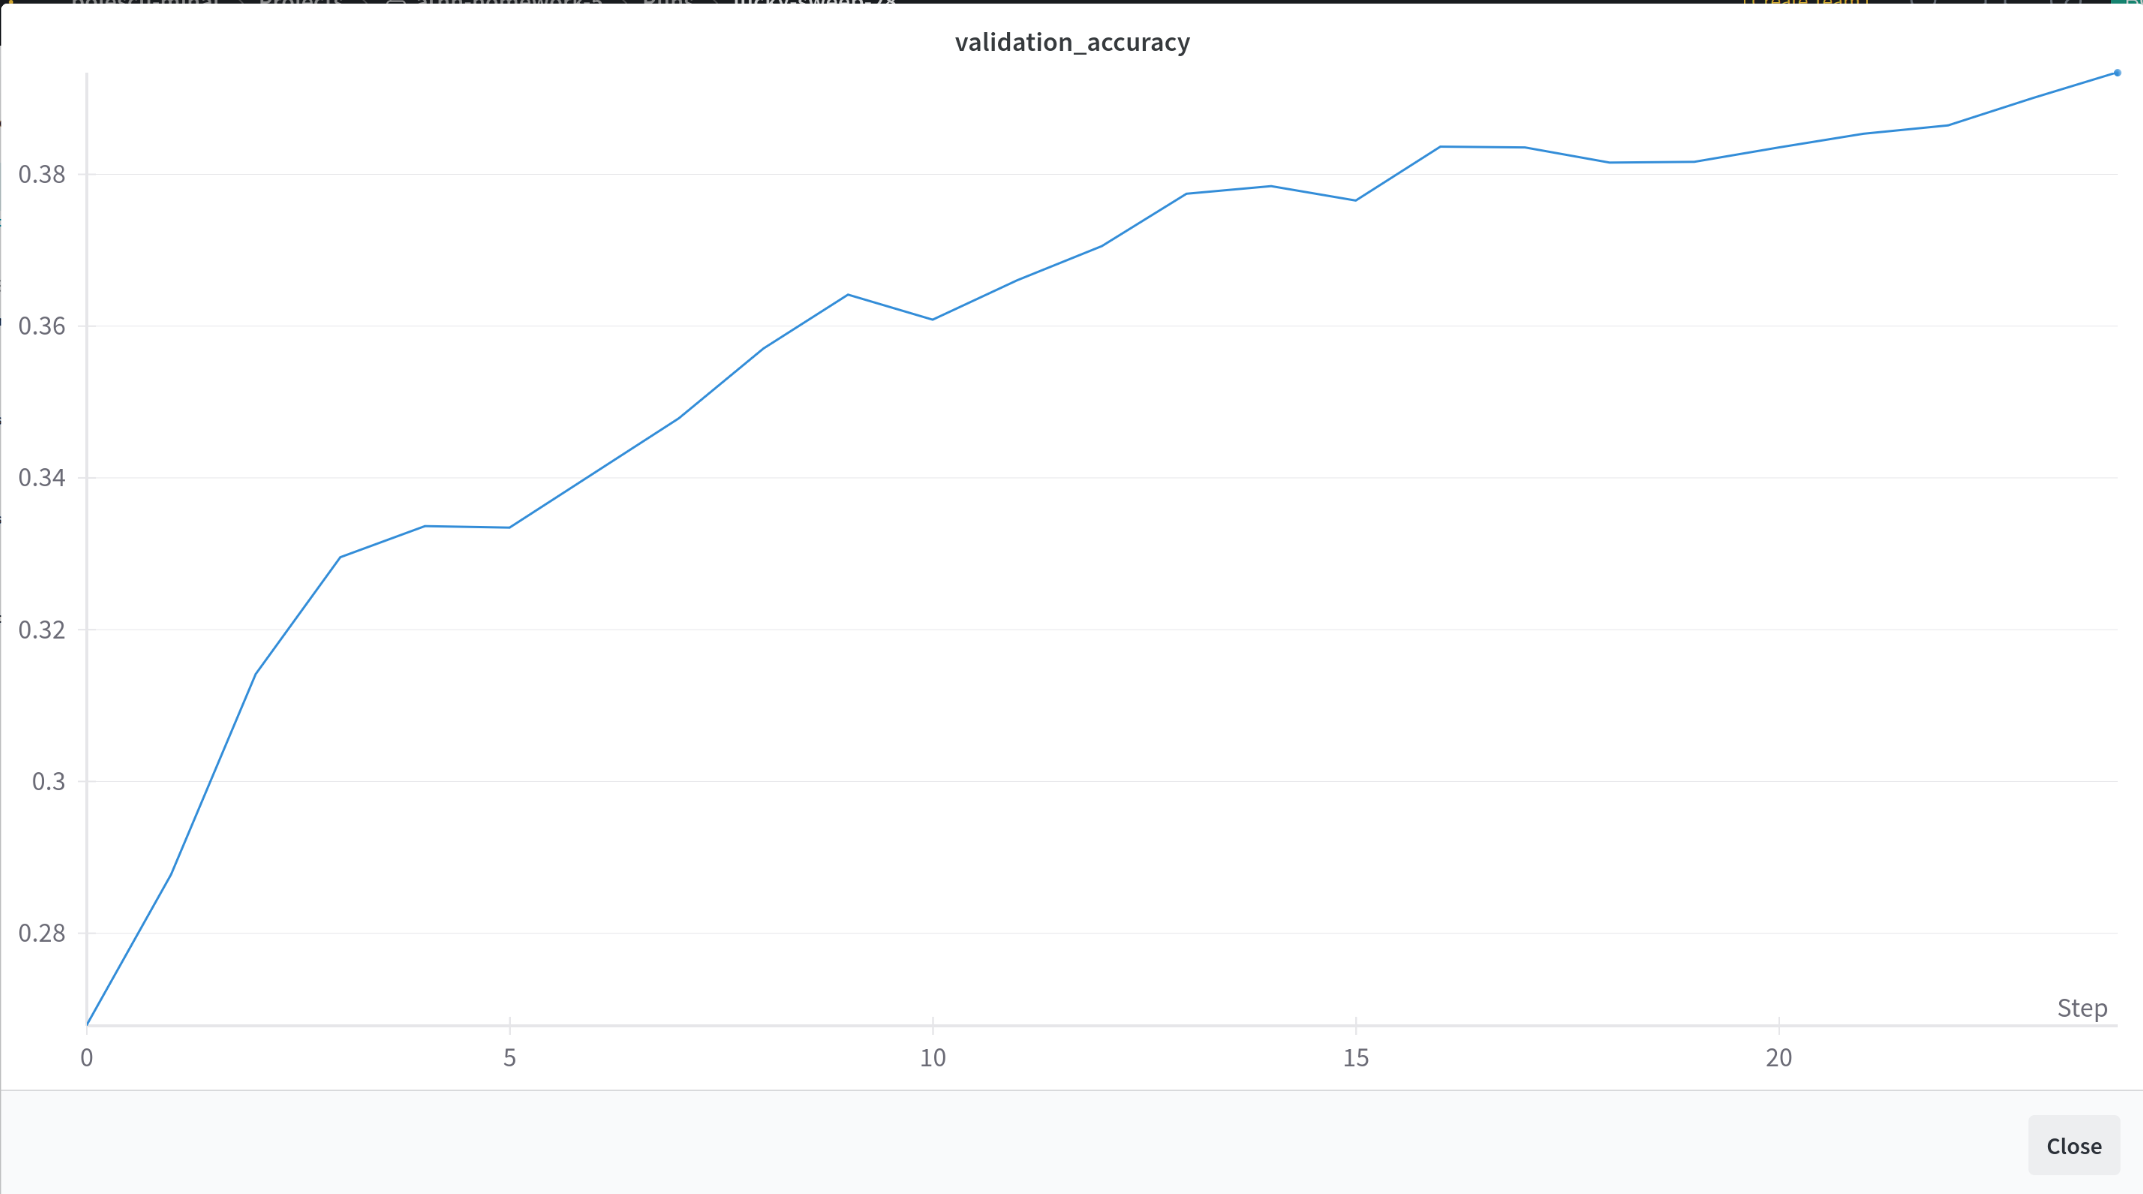
\includegraphics[width=\linewidth]{resources/previous_validation_accuracy_graph.png}
        \captionof{figure}{Validation accuracy of the previous project}
    \end{minipage}
\end{center}

\begin{center}
    \begin{minipage}{0.75\linewidth}
        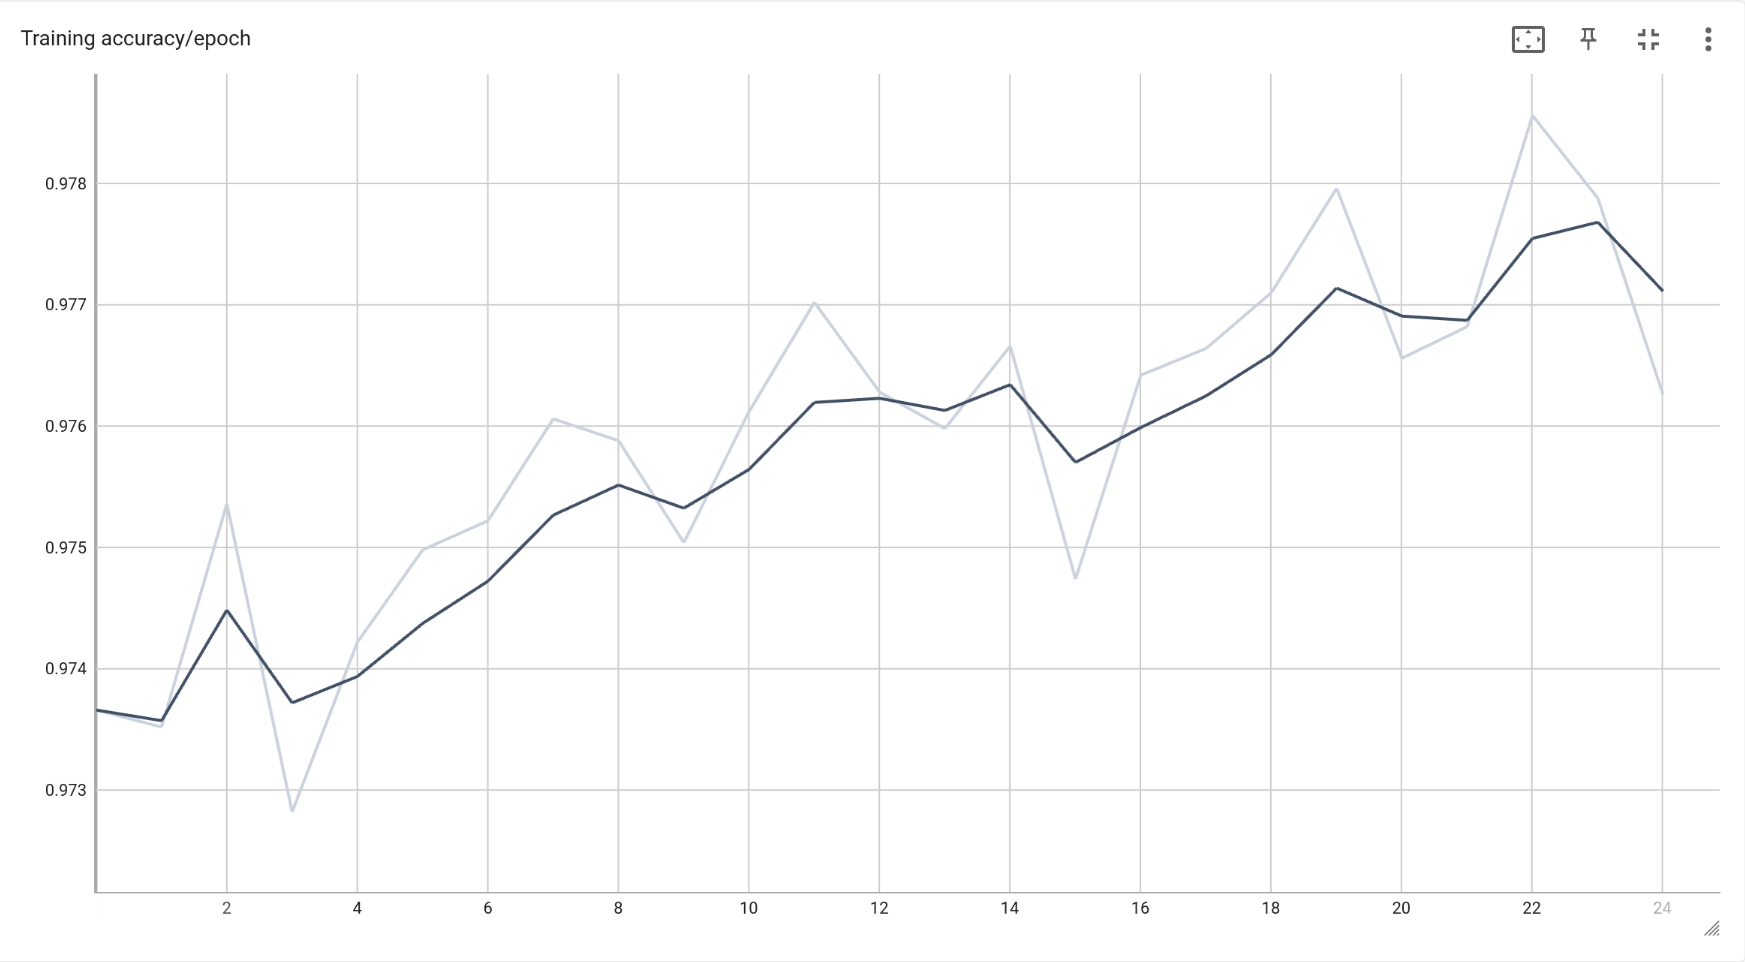
\includegraphics[width=\linewidth]{resources/validation_accuracy_graph.png}
        \captionof{figure}{Validation accuracy of the current project}
    \end{minipage}
\end{center}

The charts present the best-achieved results for each project. The difference is a staggering 38.5\%, which should prove
how important convolutional and dropout layers are.

\section{Conclusions}
Convolutional layers are quintesential to building accurate neural network models that will be used on image classification.
They are a rather time-expensive solution especially when training, but their usage pays-off compared to projects that don't
use them.

\end{document}
